% inhaltlich vollständig
% todo: Redigieren

\chapter{Methodik und Anwendungszenarien} % (fold)
\label{cha:methodik}

In diesem Kapitel wird die Methodik vorgestellt, die zur Externalisierung von mentalen Modellen im Rahmen von „Articulation Work“ zur Anwendung kommt. Die Inhalte dieses Kapitels bauen auf den Ergebnissen der Kapitel \ref{cha:articulation_work}  und \ref{cha:mentale_modelle} auf. Die Anforderungen an die Unterstützung durch ein Werkzeug, die sich aufgrund der hier vorgestellten Methodik ergeben, werden in Kapitel \ref{cha:anforderungen} identifiziert und in weiterer Folge in einem Werkzeug umgesetzt.

\begin{figure}[htbp]
	\centering
		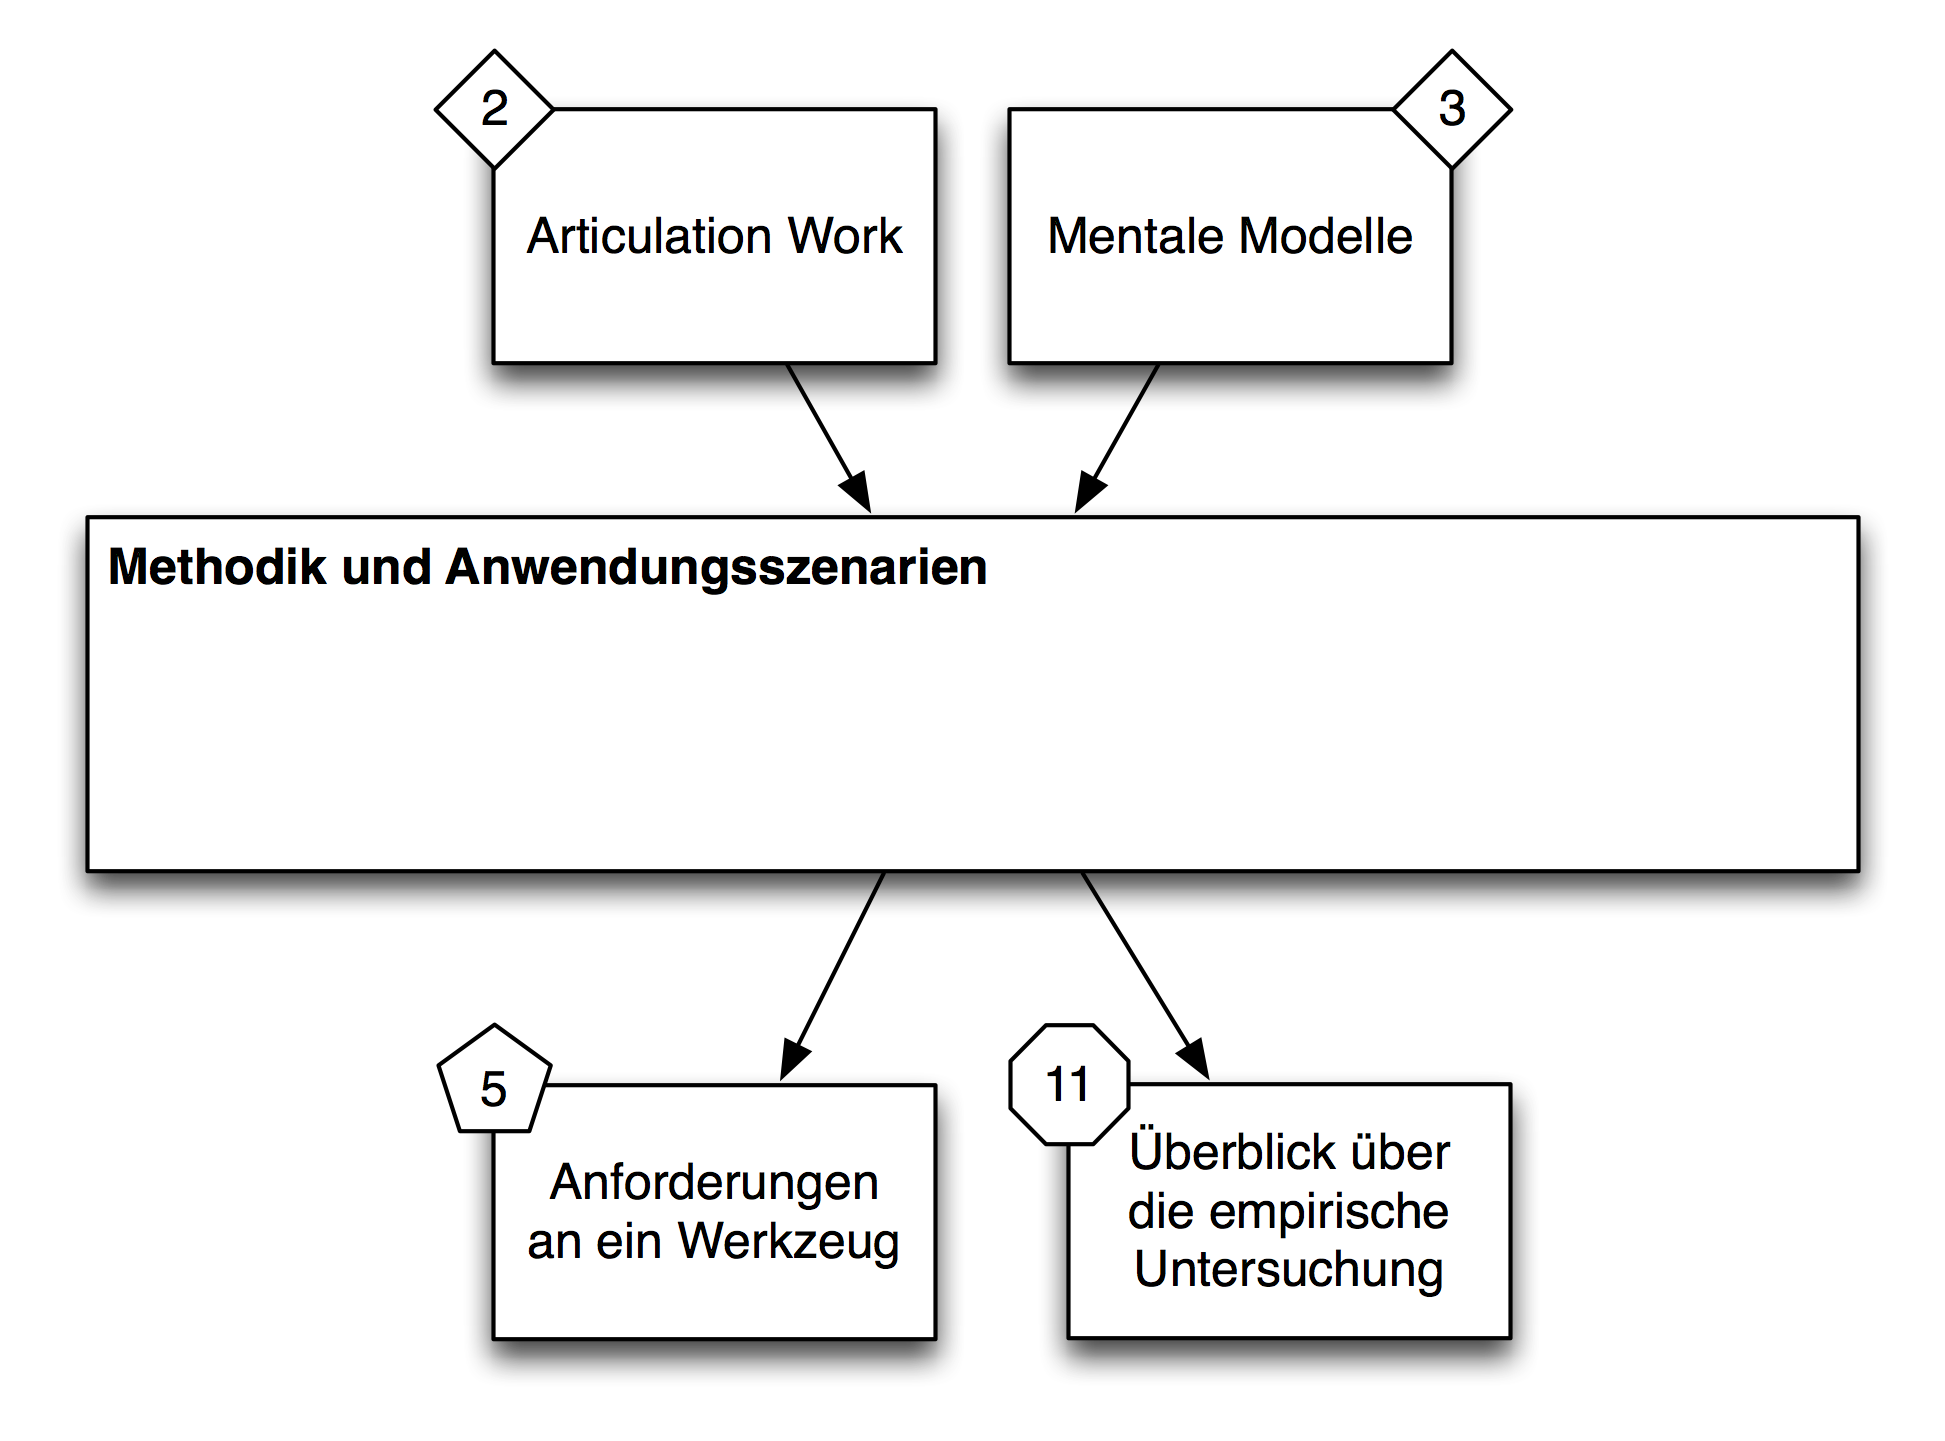
\includegraphics[scale=0.75]{img/Kontextgrafiken/k4.png}
	\caption{Kapitel „Methodik und Anwendungsszenarien“ im Gesamtzusammenhang}
	\label{fig:img_Kontextgrafiken_k4}
\end{figure}

Basierend auf den Schlussfolgerungen, die \citet{Ifenthaler06} hinsichtlich der Eignung der beschriebenen Methoden zur Externalisierung von mentalen Modellen zieht, scheinen jene Ansätze, die auf der Bildung diagrammatischer Modelle basieren, besser für die Unterstützung expliziter „Articulation Work“ geeignet zu sein als Methoden, die auf einer rein natürlichsprachlichen Repräsentation aufbauen. Dies liegt vor allem in der höheren Abstraktion begründet, die die externe Repräsentation als interindividuellen Ankerpunkt für Kommunikation besser geeignet macht. Dies deckt sich mit den Aussagen von  \citet{Sarini02}, \citet{Herrmann02}, \citet{Raposo04} oder \citet{Jorgensen04}, die aus Sicht von „Articulation Work“ für die Verwendung von (diagrammatischen) Modellen zur Unterstützung argumentieren.

Betrachtet man nun die beiden Vertreter der auf diagrammatischen Modellen aufbauenden Methoden -- Strukturlegetechniken und Concept Mapping --, so zeigt sich hinsichtlich der Eignung zum Unterstützung von „Articulation Work“ kein eindeutiger Vorteil für eine der beiden Methoden. Vielmehr weisen beide in diesem Kontext Vor- und Nachteile auf. Hier wird deshalb versucht, die Vorteile von Strukturlegetechniken -- im Wesentlichen die Unmittelbarkeit der physischen Repräsentation -- mit jenen von Concept Mapping -- der Flexibilität der Modellierung sowie der Möglichkeit der Unterstützung des Modellierungsprozesses durch Computersysteme -- zu vereinen.

Dabei wird auf das für „Articulation Work“ besser geeignete methodische Vorgehen von „Concept Mapping“ zurückgegriffen, während die Modellierungsumgebung an das bei „Strukturlegetechniken“ vorgeschlagene Szenario angepasst wird.

\section{Durchführungsrahmen} % (fold)
\label{sec:durchführungsrahmen}

Der Rahmen, in explizite „Articulation Work“ mit Unterstützung von externalisierten Modellen durchgeführt wird, ist an den Aufbau von Strukturlegetechniken angelehnt. Eine wesentliche Eigenschaft ist hierbei die physische Modellierungsoberfläche, auf der das Modell mittels real vorhandener und unmittelbar manipulierbaren Elementen aufgebaut wird. 

Im Sinne der Abstimmung unterschiedlicher Sichten muss eine kooperative, nicht exklusive Manipulierbarkeit des Modells gewährleistet sein. Das Modell selbst ist -- orientiert an der Offenheit der Repräsentation bei „Concept Mapping“ -- weder in der Art der Elemente noch der Beziehungen eingeschränkt. 

Hinsichtlich des Durchführungsrahmen ist auch die Notwendigkeit des Einsatzes einer Person zu diskutieren, die den Externalisierungsprozess anleitet und steuernd in diesen eingreift. Die Dialog-Konsens-Methode, die im Rahmen von Strukturlegetechniken zur Anwendung kommt, sieht die Rolle eines Untersuchungsleiters vor, der den Ablauf der Externalisierung strukturell anleitet. Inhaltlich hat der Untersuchungsleiter jedoch keine neutrale Rolle inne, sondern tritt im Rahmen des Dialog-Konsens-Prozesses in Interaktion mit der externalisierenden Person. Ziel des Untersuchungsleiters ist es, das mentale Modell der externalisierenden Person zu erschließen und zu verstehen. In kooperativen Situationen (die von der Dialog-Konsens-Methode nach \citep{Scheele88} nicht explizit berücksichtigt werden), wo gegenseitiges Verständnis erreicht werden muss, wechselt demnach die Rolle des Untersuchungsleiters inhaltlich gesehen dynamisch. 

Aus Sicht der Prozesssteuerung kann zu diesem Zeitpunkt nicht entschieden werden, ob ein Untersuchungsleiter benötigt wird oder nicht. Bei Strukturlegetechniken beschränkt sich dessen Aufgabe auf die Sicherstellung der Fokussierung der beteiligten Personen auf die jeweilige Aufgabe. Im Rahmen der Concept Mapping Methode ist ein intervenierender Untersuchungsleiter nicht vorgesehen. Für den hier vorgestellten Ansatz bedeutet dies, das die Rolle der Untersuchungsleiters vorerst unbesetzt bleibt, methodisch aber im Sinne der Rolle bei Strukturlegetechniken zulässig ist. 

% subsection durchführungsrahmen (end)

\section{Vorgehen} % (fold)
\label{sub:vorgehen}

Sowohl im Bereich der Strukturlegetechniken als auch im „Concept Mapping“ wird vorgeschlagen, den initialen Modellierungsprozess in zwei Phasen -- Konzeptsammlung und Konzeptstrukturierung -- zu teilen und in der Folge das Modell iterativ solange zu verändern bzw. zu erweitern, bis alle Beteiligten mit der Lösung zufrieden sind (im Bereich der Strukturlegetechniken wird die als „Dialog-Konsens“ bezeichnet, im „Concept Mapping“ spricht man von „Revisions“ des Modells, die erstellt werden müssen). Beide Abläufe sind in Abbildung \ref{fig:img_MentaleModelle_slt_cm} dargestellt.

\begin{figure}[htbp]
	\centering
		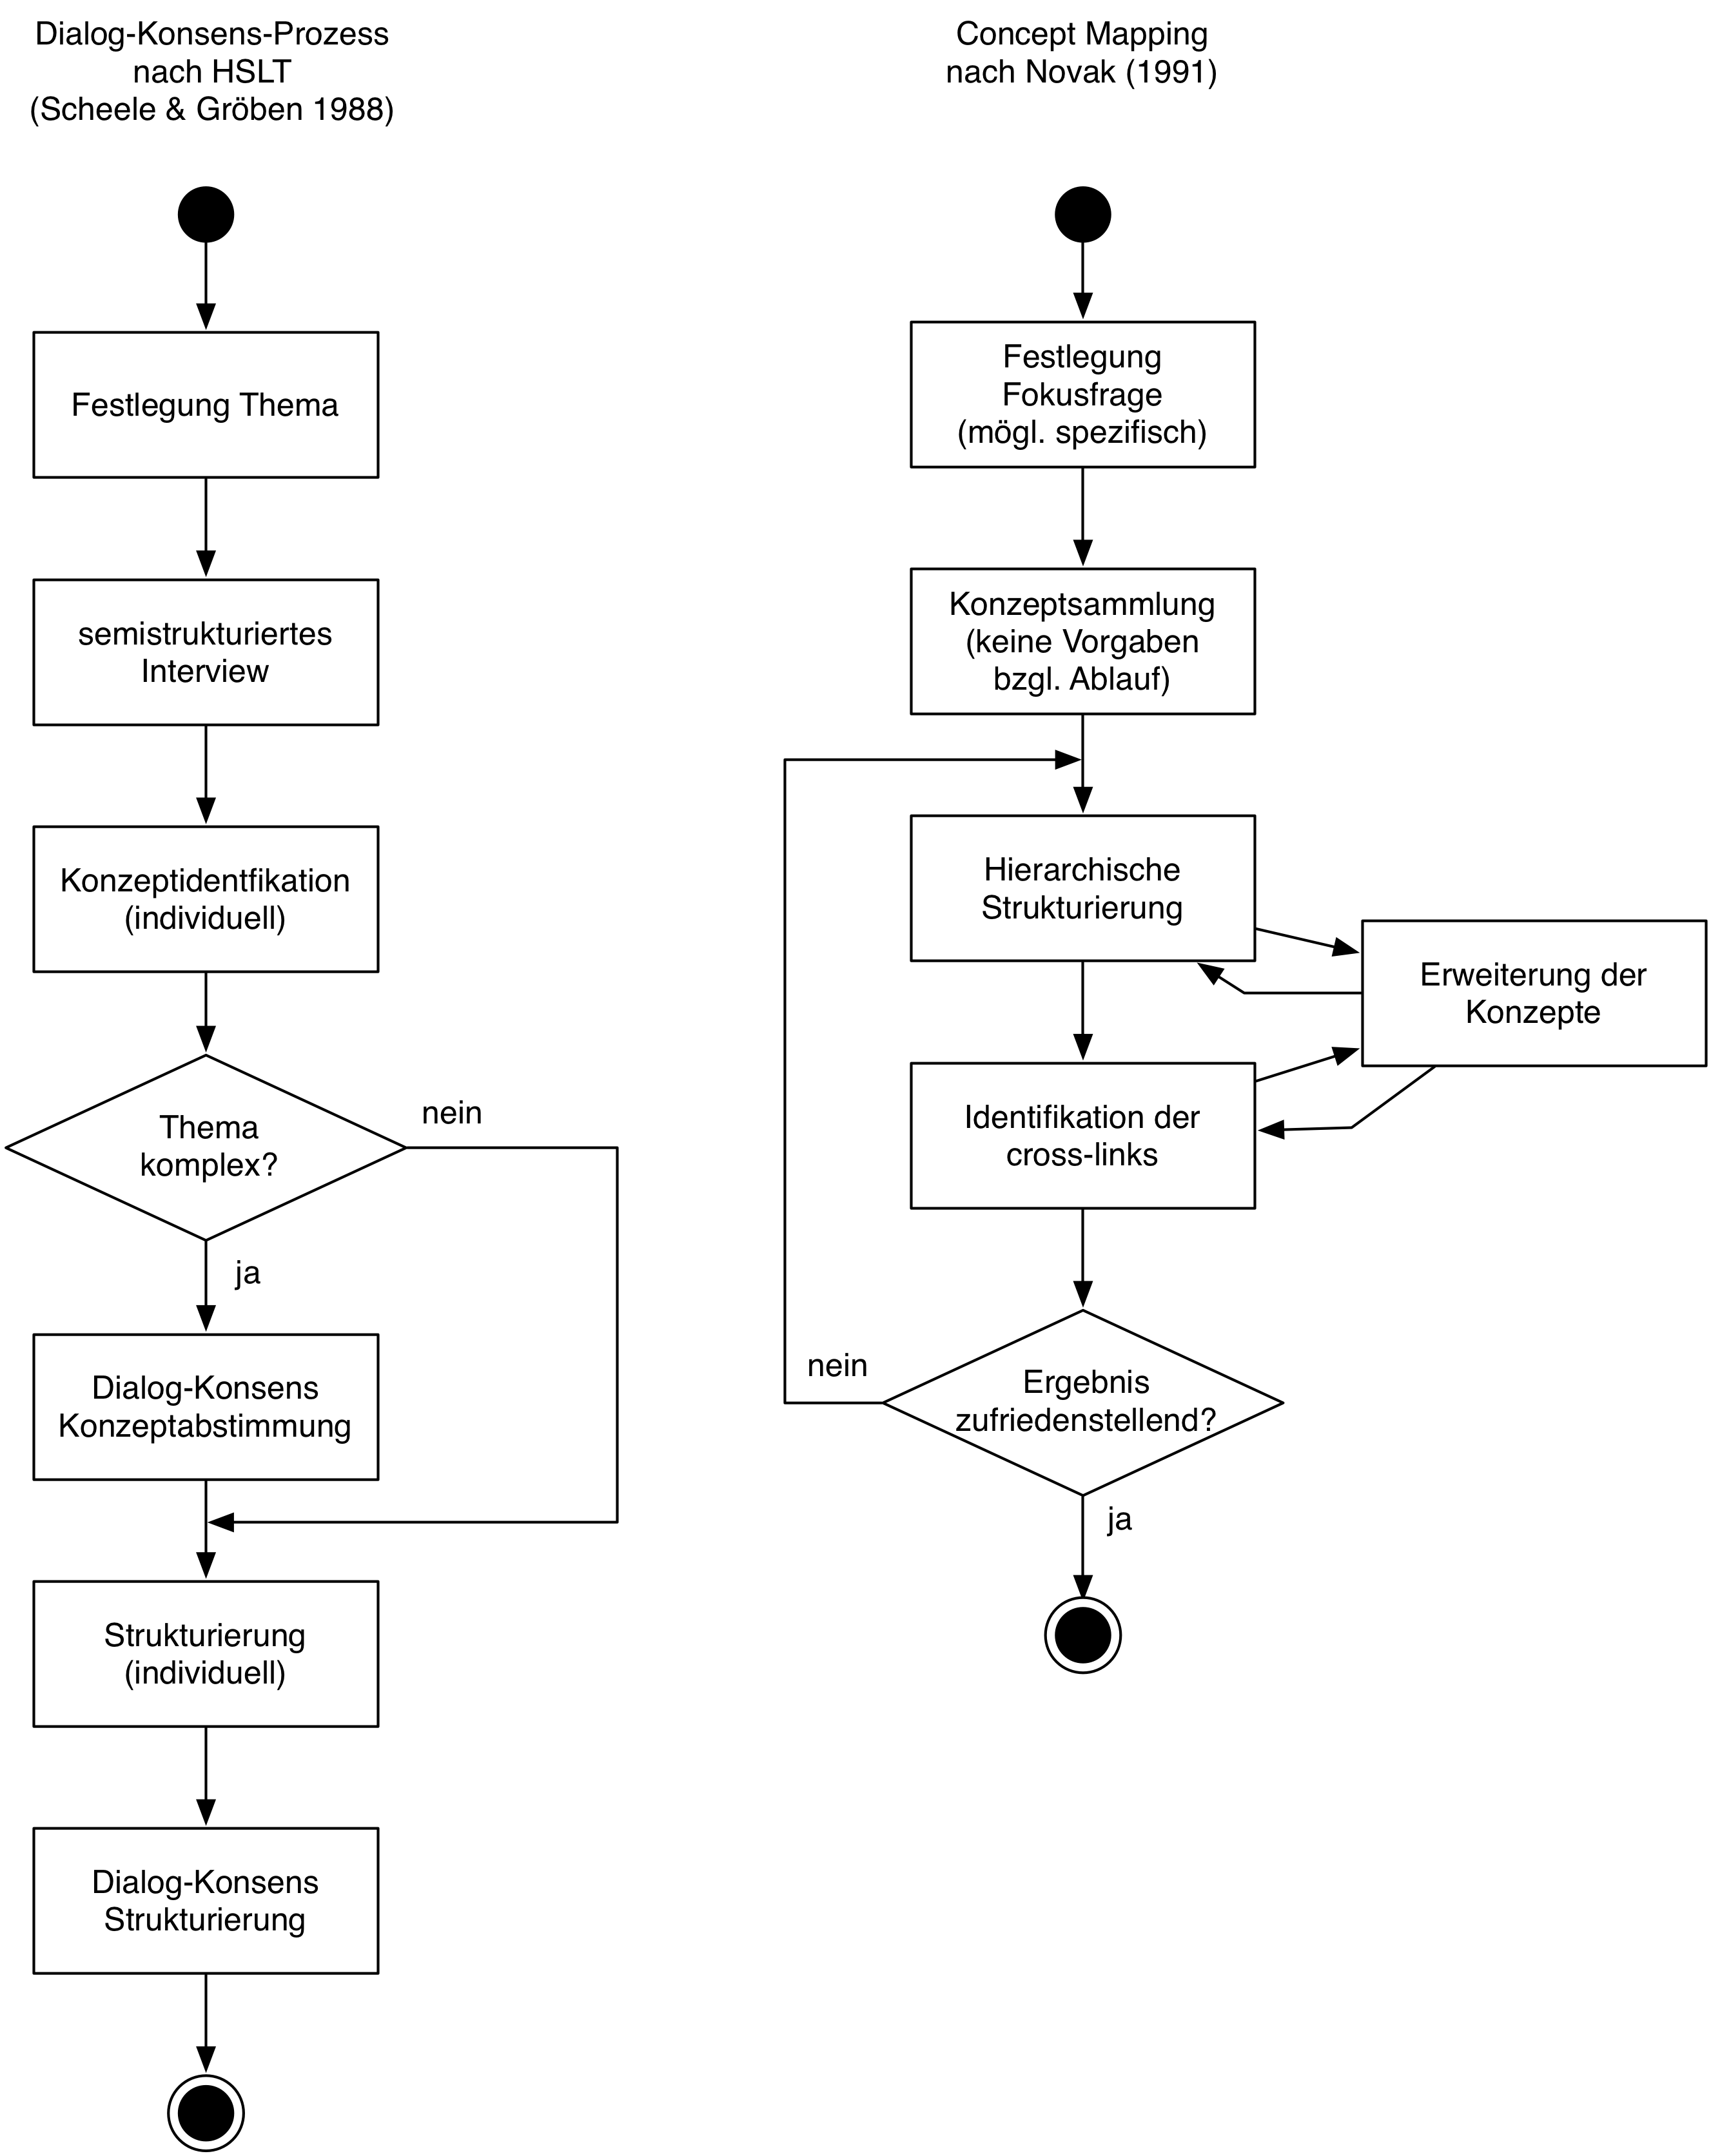
\includegraphics[width=\textwidth]{img/MentaleModelle/slt_cm.png}
	\caption{Externalisierung mentaler Modelle mittels Strukturlegetechniken und Concept Mapping}
	\label{fig:img_MentaleModelle_slt_cm}
\end{figure}

Das „Dialog-Konsens“-Vorgehen nach \citet{Scheele88} ist stark reglementiert und in den einzelnen Schritten mit definierten Methoden bzw. Vorgehensvorschriften hinterlegt. Die im Rahmen von „Concept Mapping“ vorgeschlagene Methode ist hier offener und erscheint damit für die Anwendung im Rahmen von „expliziter Articulation Work“ besser geeignet. Dies liegt am eher informellen Durchführungsrahmen von „expliziter Articulation Work“ begründet, deren Ausgestaltung individuell verschieden ist und zwischen den Beteiligten (implizit) ausgehandelt wird. Ziel ist hier, den Artikulations-Prozess zu unterstützen und nicht, ihn zu formalisieren und in vorgegebene Ablauf-Grenzen zu pressen. 

Auch die zweiphasige Durchführung des Modellierungsprozesses muss unter diesem Gesichtspunkt hinterfragt werden. Die Unterteilung in zwei Phasen erscheint bei der Beschreibung von konzeptuellen Modellen (zum „alignment of meanings“) sinnvoll. Begründet liegt dies in der Vielfalt möglicher Strukturierierungsvarianten bei dieser Art von Modellen. Im Gegensatz dazu ist die zweistufige Abhandlung der Externalisierung bei Modellen von Abläufen (bei „alignment of procedures“) nur bedingt sinnvoll, da Aktivitäts-Konzepte im Normalfall bereits in deren kausalen Abfolge externalisiert und dann bzw. parallel mit zusätzlichen Konzepten hinterlegt werden. Die Verwendung dieser Form von Modellen ist bei der Abstimmung von Arbeit gängig, wird aber weder bei Concept Mapping noch bei Strukturlegetechniken explizit angesprochen. Insofern ist die explizite Durchführung der ersten Phase -- also der Konzeptsammung -- als optional anzusehen. Im Sinne der Methode zur Erstellung von Concept Maps nach \citet{Novak06} werden Konzeptsammlungs-Phasen in den iterativen Modellverfeinerungsprozess eingeflochten, wenn dies in der Situation als notwendig erscheint.

Die im Folgenden beschriebene Methodik basiert wie oben angeführt auf den in Kapitel \ref{cha:mentale_modelle} vorgestellten Methoden „Strukturlegetechniken“ und „Concept Mapping“. Für die Anpassung an den Durchführungskontext im Rahmen von „Articulation Work“ wurden jene in Abschnitt \ref{sec:unterstützung_von_articulation_work} beschriebenen Ansätze zur Unterstützung von „Articulation Work“ herangezogen, die Aussagen zu den Anforderung eine eine Methodik treffen. Im Einzelnen sind dies \citet{Corbin93}\footnote{beschrieben auf Seite \pageref{steps:corbin} in dieser Arbeit}, \citet{Jorgensen04}\footnote{beschrieben auf Seite \pageref{steps:jorgensen}}, \citet{Cabitza06}\footnote{beschrieben auf Seite \pageref{steps:cabitza}} sowie \citet{Herrmann02}\footnote{beschrieben auf Seite \pageref{steps:herrmann}}. Letztere Arbeit spezifiziert aber vor allem Anforderungen an eine etwaige Werkzeugunterstützung, weshalb sie in Kapitel \ref{cha:anforderungen} nochmals näher berücksichtigt wird.

Die einzelnen Schritte, die bei der Anwendung der Methodik zur Anwendung kommen, sind im Einzelnen:
\begin{itemize}
 \item Einarbeitung
 \item Konzeptsammlung 
 \item Konzeptstrukturierung
 \item Restrukturierung
\end{itemize}

Diese Aufzählung gibt keine Reihenfolge der durchzuführenden Schritte vor. Vielmehr sind die einzelnen Blöcke als Module zu sehen, die je nach Anwendungsfall zu einem beliebigen Zeitpunkt im Externalisierungsprozess (auch mehrfach) zur Anwendung kommen oder auch entfallen können. Im Folgenden wird die Durchführung der einzelnen Schritte kurz umrissen und angegeben, in welchen Situationen deren Einsatz angemessen bzw. notwendig erscheint.

\subsection{Einarbeitung}

Die Einarbeitung wird nach Bedarf durchgeführt, wenn zumindest eine Person nicht mit der Methodik oder dem unterstützenden Werkzeug vertraut ist. Im Rahmen einer Erklärungsphase wird den Teilnehmern die Funktionalität des Werkzeugs vorgestellt und dessen Verwendung im Rahmen der Methodik dargelegt. Dies erfolgt durch eine Person, die sowohl mit dem Werkzeug als auch der Methodik vertraut ist. Neben einem etwaigen Untersuchungsleiter kann diese Rolle auch durch einen anderen Teilnehmer wahrgenommen werden, der bereits eine Externalisierung mit Unterstützung der Methodik und des Werkzeugs teilgenommen hat.

Der Erklärungsphase kann auch eine freie Experimentier-Phase angeschlossen werden, in der die Teilnehmer die Gelegenheit haben, ohne Vorgaben das Werkzeug zu verwenden und dessen Funktionalität zu erfassen. Nach Bedarf kann dazu auch ein exemplarisches Thema vorgegeben werden, anhand dessen die Durchführung der Methodik gezeigt bzw. durchgespielt werden kann.

Zu beachten ist im Rahmen der Einarbeitung, dass die Offenheit der Methodik nicht unbeabsichtigt eingeschränkt wird, indem durch Erklärungen oder Beispiele strukturelle oder inhaltliche Vorgaben gemacht werden, an denen sich die Teilnehmer in der Folge bei der Durchführung der Externalisierung orientieren. Strukturell betrifft dies etwa Vergleiche mit unter Umständen bekannten Methoden wie „Mind Mapping“, dessen hierarchischer Aufbau jedoch nicht die Offenheit der Strukturen zulässt, die in der vorliegenden Arbeit möglich und notwendig sind. Inhaltliche Einschränkungen können etwa durch Beispiele von Konzeptklassen vorgegeben werden, die von den Teilnehmern unreflektiert übernommen werden und die dadurch die semantische Offenheit der Repräsentation einschränken.

\subsection{Konzeptsammlung}

Bei der Sammlung der Konzepte wird neben den im Rahmen von „Concept Mapping“ und Strukturlegetechniken vorgeschlagenen Vorgehen eine weitere Einschränkung vorgenommen, die aus den Erkenntnissen der Forschung im Bereich der „Articulation Work“ stammt. Sowohl „Concept Mapping“ als auch Strukturlegetechniken führen keine explizite inhaltliche Klassifizierung der gesammelten Konzepte durch -- es werden keine Klassen von Konzepten gebildet, die einen gemeinsamen Aspekt oder Bezugspunkt aufweisen. Während „Concept Mapping“ eine derartige Strukturierung zumindest zulässt, ist diese bei Strukturlegetechniken nicht vorgesehen.

Bereits Strauss spricht von den „salient dimensions of work“ \citep[][S.5]{Fjuk97}, die im Rahmen von „Articulation Work“ abgestimmt werden müssen und deren Wichtigkeit für die jeweils beteiligten Individuen von Anwendungsfall zu Anwendungsfall verschieden sein kann. Auch \citet{Sarini02} unterstützen mit ihrer Arbeit die Abstimmung unterschiedlicher Perspektiven auf einen Arbeitsablauf anhand der Identifikation gemeinsamer Konzeptklassen und deren Ausprägungen. Die Ebene der Konzeptklassen scheint also im Rahmen von „Articulation Work“ eine nicht unwesentliche Rolle zu spielen. Sie werden in der hier vorgeschlagenen Methodik deshalb explizit berücksichtigt. 

Dazu sind zwei Vorgehensweisen vorstellbar. Einerseits kann ein Satz an domänen- bzw. anwendungsspezifischen Konzeptklassen vorgegeben werden, der von den Benutzern verwendet werden muss. Anderseits können die Konzeptklassen selbst Gegenstand von „Articulation Work“ sein und erst während dem Externalisierungsvorgang festgelegt werden. Diese Variante erscheit im Anwendungsgebiet von „Articulation Work“ besser geeignet, da sie die Denkstrukturen der beteiligten Individuen auf mehreren Ebenen offenlegt. Unerfahrene Benutzer können mit der Offenheit des Ansatzes jedoch überfordert sein, was sich darin äußert, dass keine oder sehr allgemeine, umfassende Konzeptklassen ohne Unterscheidungskraft gebildet werden. Ein möglicher Lösungsansatz ist hier die Kombination der beiden beschriebenen Ansätze, indem eine Kernsatz an domänenspezifischen Konzeptklassen vorgegeben wird, gleichzeitig aber eine Erweiterung durch individuelle Konzeptklassen ermöglicht wird. Diese Variante ist in \citet{Oppl05} hinsichtlich ihrer Durchführung und Auswirkungen beschrieben. 

\subsection{Konzeptstrukturierung}

Die Konzeptstrukturierung erfolgt in der hier beschriebenen Methodik entsprechend dem Vorgehen bei „Concept Mapping“ vollständig offen, d.h. dass keine semantisch vordefinierten Arten von Beziehungen verwendet werden. Anwender sind in der Bezeichnung der Beziehungen vollkommen frei und können diese auch explizit nicht bezeichnen, wenn ihnen dies nicht notwendig erscheint (als Abweichung zum „Concept Mapping“). Syntaktisch sind Beziehungen immer binär, haben also nur zwei Endpunkte und können ungerichtet, gerichtet oder bidirektional sein. Die Einschränkung auf binäre Beziehungen gegenüber „Concept Mapping“ wird basierend auf den Annahmen bei Strukturlegetechniken getroffen. Dort werden grundsätzlich binäre Zusammenhänge verwendet, da diese eindeutiger erfassbar sind. Beziehungen mit mehr als zwei Endpunkten sind oft mehrdeutig und anfällig für Missinterpretation.

Vor der Festlegung von Beziehungen erfolgt in der hier beschriebenen Methode (analog zu Strukturlegetechniken) die initiale Strukturierung der Konzepte durch räumliche Anordnung derselben auf der physischen Modellierungsoberfläche. Bereits dabei kann in die Position der Konzepte Bedeutung codiert werden. So ist es möglich, rein durch die Positionierung Hierarchien oder Kausalzusammenhänge anzudeuten. Die Methodik macht hier keine Vorgaben, lässt aber diese Form der Bedeutungsfestlegung explizit zu. Für das resultierende Modell hat dies die Auswirkung, dass dessen Semantik nicht ausschließlich in dessen Netzwerkgraphen codiert ist, die Erfassung der Bedeutung der Knoten (Konzepte) und Kanten (Beziehungen) alleine also nicht ausreicht. Vielmehr muss auch die exakte Positionierung der Knoten (Konzepte) in die Repräsentation des Modells mit aufgenommen werden. Zur Rekonstruktion des Modells ist dies ohnehin notwendig, an dieser Stelle geht die Bedeutung der Position jedoch weiter und codiert für sich stehend semantisch hinterlegte Zusammenhänge. 

\subsection{Restrukturierung}

Unter Restrukturierung wird hier die Neuanordnung von bereits verwendeten Konzepten auf der Modellierungsoberfläche verstanden. Wie zuvor erwähnt ist in den Positionen der Konzepte oft Information über deren Beziehung zueinander codiert. Neben der Veränderung von explizit hergestellten Verbindungen zwischen Konzepten ist so auch durch Veränderung der Konzept-Positionen eine Änderung der Modellbedeutung möglich. Zweiteres kommt im Kontext von „Articulation Work“ vor allem dann zum Tragen, wenn der wahrgenommene Kontext von Arbeitsabläufen abgebildet wird und dieser zwischen mehreren Personen ausgehandelt wird (vgl. \citep{Wahlmuller10} bzw. Kapitel \ref{cha:eval_modell}). Dabei werden Konzepte im Rahmen ihrer (wahrgenommen) Bedeutung für den Arbeitsablauf in bzw. um diesen an- und umgeordnet und spezifizieren so dessen Durchführungsrahmen näher aus. 

Die Restrukturierung kann sich auch auf eine Veränderung der explizit angegebenen Verbindungen zwischen Konzepten beziehen. Im Gegensatz zu einer Veränderung der räumlichen Anordnung der Konzepte müssen in diesem Fall die betreffenden Verbindungen entfernt werden und entsprechend neue hinzugefügt werden. In beiden Fällen ist es in Hinblick auf eine Werkzeugunterstützung wichtig, die Durchführung experimenteller Veränderungen zu ermöglichen, die einfach rückgängig gemacht werden können. Dazu ist es notwendig, bestimmte Modellzustände als Referenz kennzeichnen zu können, die in der Folge als Bezugspunkte für eine allfällige Wiederherstellung dienen können.

% section vorgehen (end)

\section{Anwendungsszenarien}

Die eben beschriebenen Schritte bei der Anwendung der Methodik sind, wie bereits erwähnt, als Bausteine zu verstehen, die je nach Anwendungsszenario unterschiedlich zusammengesetzt werden können oder auch wegfallen können. Außerdem ist jeweils eine individuelle oder kooperative Anwendung möglich. Auch diese Entscheidung ist vom jeweiligen Anwendungszenario abhängig.

In der Folge werden nun exemplarisch einige mögliche Anwendungsszenarien der Methodik beschrieben, die sich aus dem Einsatz derselben im Rahmen von „Articulation Work“ ableiten lassen. Neben den beschriebenen Szenarien sind aufgrund der Offenheit der Methodik auch weitere Anwendungsvarianten denkbar. Im Rahmen von „Articulation Work“ treten folgende Einsatzszenarien auf:

\begin{itemize}
 \item Verfeinerung mentaler Modelle
 \item Wissenstransfer
 \item Abstimmung mentaler Modelle 
 \item Aushandlung mentaler Modelle
\end{itemize}

Diese Szenarien wurden auch im Rahmen der Evaluierung in unterschiedlichen Anwendungsblöcken abgebildet (siehe Kapitel \ref{cha:eval_ueberblick}) und dienen als Grundlage der empirischen Überprüfung der dort formulierten Hypothesen.

\subsection{Verfeinerung mentaler Modelle} % (fold)
\label{sub:verfeinerung_individueller_mentaler_modelle}

Die Verfeinerung mentaler Modelle ist ein Anwendungsfall einer nicht kooperativen, ausschließlich individuellen Anwendung der Methodik. Die „Articulation Work“, in deren Rahmen die Externalisierung durchgeführt wird, hat reflexiven Charakter und dient der Vertiefung des Verständnisses eines realen Phänomens. Ziel ist es, die beobachteten Abläufe oder Ereignisse besser erklären zu können, um so letztendlich adäquatere Handlungsalternativen ableiten zu können. Die Aufgabenstellung lautet dementsprechend, das aktuelle Verständnis des Phänomens zu externalisieren und in der Folge anhand der externalisierten Repräsentation nach möglicherweise veränderten oder erweiterbaren Erklärungsansätzen zu suchen (siehe dazu die Beschreibung des Ansatzes von \citet{Fjuk97} in Abschnitt \ref{sub:arten_fjuk}).

Bestehen keine Vorkenntnissen des Individuums in der Durchführung der Methodik bzw. der Verwendung der Werkzeugunterstützung, so wird die Aktivität „Einarbeitung“ durchgeführt. Dies ist in diesem Szenario der einzige Punkt, an dem eine zweite Person (also ein „Prozessbegleiter“) eingreift. In den späteren Phasen -- der eigentlichen Externalisierung -- ist lediglich das betreffende Individuum beteiligt.

Je nach individueller Präferenz beginnt der eigentliche Externalisierungsvorgang mit einer dedizierten Konzeptsammlungsphase oder einer bereits von Beginn an verwobenen Sammlungs- und Strukturierungsphase. Auch bei Beginn mit einer Konzeptsammlungsphase geht die darauf folgende Strukturierungsphase mit einer iterativ verwobenen Ergänzung bzw. Veränderung der Konzepte einher. Der erste Teil der Anwendung ist abgeschlossen, wenn die initiale externalisierte Repräsentation den wahrgenommenen Ist-Zustand für das Individuum abbildet.

Im zweiten Teil wird die externalisierte Repräsentation als Grundlage für eine tiefergehende Erklärung des realen Phänomens herangezogen. Im Rahmen dieses reflexiven Prozesses kann es zu Restrukturierungen im Modell kommen, um dessen Ausdrucksstärke oder Erklärungskraft zu verbessern. Dies kann Ergänzungen (wie etwa die Berücksichtigung von Ausnahme- oder Spezialfällen) umfassen aber auch zu einer grundlegenden Veränderung des ursprünglichen Erklärungsansatzes führen (siehe „Assimilation“ vs. „Akkommodation“ in Abschnitt \ref{sec:begriffsbestimmung} bzw. die Unterscheidung zwischen „single-loop learning“ und „double-loop learning“ bei \citet{Argyris76}).

Die Anwendung der Methodik ist abgeschlossen, wenn für das Individuum ein konsistenter mentaler Zustand erreicht ist (das Erklärungsmodell also als konsistent wahrgenommen wird). Dies kann auch der ursprüngliche Ausgangszustand sein, der durch die Externalisierung betätigt und weiter gefestigt wurde. Bei einer Veränderung des mentalen Modells muss sich dieses in der Folge in der praktischen Anwendung bei der Entwicklung von Handlungsalternativen bei der Konfrontation mit dem gegebenen Phänomen in der realen Welt bewähren (im Sinne des „assess“ im \gls{OADI}-Zyklus des individuellen Lernens bei \citet{Kim93}). Die Anwendung der Methodik dient hier also der Entwicklung neuer Erklärungsansätze und Handlungsalternativen, deren Bestätigung und Festigung erfolgt erst in der praktischen Anwendung.

% subsection verfeinerung_individueller_mentaler_modelle (end)

\subsection{Wissenstransfer} % (fold)
\label{sub:wissenstransfer}

Das Szenario „Wissenstransfer“ bezieht sich auf Situationen, in denen Wissen von einer Person an ein oder mehrere Individuen weitergegeben werden muss. Im Rahmen von „Articulation Work“ kann diese Situation auftreten, wenn ein Arbeitsablauf von manchen Beteiligten aufgrund von mangelnder Erfahrung oder Unkenntnis als problematisch wahrgenommen wird, zumindest eine Person aber das Faken- oder Handlungswissen besitzt, um adäquate Handlungsalternativen ableiten zu können (siehe hier etwa den Übergang von „invisible work“ zu „visible work“ in der Beschreibung des Ansatzes von \citet{Hampson05} in Abschnitt \ref{sub:arten_hampson}). Ziel ist hier, das relevante Wissen von der kompetenten Person zu den unerfahrenen Persone zu transferieren, diese also „lernen“ zu lassen. Die Aufgabenstellung lautet dementsprechend, die relevanten Konzepte und Beziehungen zur Erklärung der Situation und der Ableitung von Handlungsalternativen durch das kompetente Individuum zu externalisieren. Aufbauend auf der externalisierten Repräsentation wird eine kooperative Reflexionsphase durchgeführt. 

Der erste Teil der Durchführung entspricht im Wesentlichen dem im ersten Szenario beschriebenen Vorgehen. Die Konzeptsammlung und -strukturierung erfolgt initial individuell, wobei die „lernenden“ Individuen an diesem Teil des Prozesses bereits beobachtend teilnehmen können. Die externalisierende Person kann den Externalisierungsprozess durch Anwendung der Prinzipien der „Methode des lauten Denkens“ (siehe Abschnitt \ref{sub:methode_des_lauten_denkens}) nachvollziehbarer machen. 

Der kooperative Teil der der Durchführung beginnt mit einer Erklärungs- und Reflexionsphase, der die externalisierte Repräsentation zugrunde liegt und als Bezugs- und Ankerpunkt dient. Je nach Verlauf des Prozesses kann diese Reflexion in eine (Re-)Strukturierungsphase übergehen, in der die Repräsentation bei punktuell auftretenden Verständnisschwierigkeiten verfeinert bzw. konkretisiert werden kann. 

Der Prozess ist abgeschlossen, wenn sowohl die „lernenden“ Individuen die als problematisch wahrgenommene Situation für sich auflösen können und auch das externalisierende Individuum den Eindruck gewinnt, dass die zu vermittelnden Konzepte von den „Lernenden“ akkommodiert wurden. Der tatsächliche Erfolg des Wissenstransfers zeigt sich wiederum erst in der praktischen Durchführung von Handlungen in der fraglichen Situation bzw. deren Auswirkungen in der Realität.

% subsection wissenstransfer (end)

\subsection{Abstimmung mentaler Modelle} % (fold)
\label{sub:abstimmung_individueller_mentaler_modelle}

Die Abstimmung mentaler Modelle ist das erste Szenario in den eine tatsächlich kooperative Externalisierung vorgenommen wird. Im Rahmen von „Articulation Work“ tritt diese Variante dann auf, wenn etablierte, individuelle bzw. lokale Arbeitsabläufe existieren, die aufgrund von neuen Anforderungen oder Rahmenbedingungen so abgestimmt werden müssen, dass sie interoperabel bzw. kooperativ durchführbar sind. Dies ist der im Rahmen von „Articulation Work“ am häufigsten genannte Anwendungsfall, auf den auch Strauss bereits in seinen ersten Arbeiten Bezug nimmt.

Ziel ist hier, die individuellen Arbeitsabläufe und deren wahrgenommene Rahmenbedingungen soweit offen zu legen, dass eine Identifikation der Schnittstellen zwischen den einzelnen Teilen und die Etablierung eines kooperativen Arbeitsablaufs möglich wird. Alternativ kann dieses Szenario auch dann auftreten, wenn ein organsiational spezifizierter Soll-Prozess den tatsächlichen Arbeitsabläufen gegenüber gestellt werden soll bzw. aus diesen ein Soll-Prozess entwickelt werden soll. Die Aufgabenstellung lautet in allen Fällen im ersten Schritt, die individuellen Beiträge zu dem angepeilten kooperativen Arbeitsablauf zu identifizieren und soweit zu externalisieren, dass diese für die anderen beteiligten Individuen erfassbar werden (im Falle der Existenz eines organisationalen Soll-Prozesses wird diese durch ein die Organisation repräsentierendes Individuum eingebracht). Im zweiten Schritt erfolgt eine kooperative Abstimmung der individuellen Beiträge, im Rahmen derer der globale Ablauf ausgehandelt wird bzw. potentielle Konfliktstellen identifiziert bzw. beseitigt werden.

Das Szenario ist grundsätzlich kooperativ und baut im ersten Teil auf den beiden zuvor beschriebenen Szenarien auf. Dies bedeutet konkret, dass die Externalisierung der individuellen Beiträge wie in Szenario 2 geschildert zwar jeweils von den einzelnen Teilnehmern separat durchgeführt wird, dass zum Zwecke der Verständlichkeit die anderen beteiligten Personen beobachtend teilnehmen können. Die individuellen Beiträge müssen dabei nur soweit offengelegt werden, wie sie die möglichen Schnittstellen im zu entwickelnden gemeinsamen Arbeitsablauf betreffen -- nicht jedes teilnehmende Individuum muss ein detailliertes mentales Modell der gesamten durchzuführenden Arbeit haben bzw. entwickeln. In Arbeitsabläufen, in denen die möglichen Kooperations-Stellen nicht abschätzbar sind, kann eine selektive Externalisierung jedoch problematisch sein. In diesem Fall müssen die individuellen Beiträge iterativ bei der kooperativen Zusammenführung soweit detailliert werden, dass eine Festlegung der Zusammenarbeit möglich wird.

Nach der Externalisierung der individuellen Beiträge folgt im zweiten Teil eine kooperative Phase, in der aufbauend auf den individuellen Beiträgen die Konzeptsammlung und -strukturierung auf globaler Ebene durchgeführt wird. Sofern sichergestellt ist, das die teilnehmenden Individuen in der ersten Phase ein Verständnis über die sie betreffenden Arbeitsbeiträge entwickelt haben, kann diese Abstimmung auf abstrakterer Ebene erfolgen. Dies bedeutet, dass die gemeinsame Externalisierung nicht auch die gesammelten individuellen Beiträge enthält, sondern sich lediglich auf diese bezieht und in der Repräsentation vorrangig die Schnittstellen und Interaktionsabläufe abgebildet werden. In dieser Phase können Sammlung, Strukturierung und Restrukturierung ggf. ineinander fließen bzw. nicht klar abgegrenzt werden. Durch die bereits gegebenen Repräsentationen der individuellen Beiträge ist eine Ausgangsbasis vorhanden, die im Rahmen der Abstimmung einen raschen Wechsel zwischen den einzelnen Aktivitäten ermöglich.

Der Prozess ist abgeschlossen, wenn alle teilnehmenden Individuen ihre Sichtweisen auf den gesamten Arbeitsablauf soweit abgestimmt haben, dass eine Durchführung desselben möglich ist. Unmittelbar kann dies nur durch die Rückmeldung der persönlichen Wahrnehmung und Eindrücke der Teilnehmer überprüft werden. Die tatsächlichen Auswirkungen auf die Arbeitspraxis -- im konkreten Fall die Etablierung oder Veränderung eines kooperativen Arbeitsablaufs -- kann wiederum nur während der Durchführung im Rahmen der „Production Work“ beurteilt werden.

% subsection abstimmung_individueller_mentaler_modelle (end)

\subsection{Aushandlung mentaler Modelle} % (fold)
\label{sub:aushandlung_individueller_mentaler_modelle}

Im Gegensatz zu den übrigen Szenarien geht das hier beschriebene Szenario nicht von etablierten, gefestigten mentalen Modellen oder existierenden Arbeitsabläufen aus. Vielmehr werden hier von Beginn an kooperativ mentale Modelle zu einer gegebenen Fragestellung entwickelt und reflektiert. Im Rahmen von „Articulation Work“ treten diese Situation vor allem dann auf, wenn ein kooperativer Arbeitsablauf neu geplant werden muss, ohne dass dieser zuvor von den beteiligten Personen als Ganzes oder in Teilen durchgeführt wurde (siehe dazu die Ausprägung „working out original arrangements“ in der Beschreibung des Ansatzes von \citet{Corbin93} in Abschnitt \ref{sec:arten_von_articulation_work}). 

Ziel ist es, auf Basis der individuellen Vorkenntnisse und Erfahrungen einen kooperativen Arbeitsablauf bzw. dessen Durchführungskontext auszuhandeln. Die Aufgabenstellung lautet dementsprechend, eine Externalisierung zu entwickeln, die den kooperativen Ablauf, die benötigten Rahmenbedingungen und ggf. den Aspekt der Arbeitsteilung abbildet. 

Dieses Szenario ist in der Durchführung der Methodik flexibel. Im Vergleich zu den anderen beschriebenen Szenarien sind individuelle Externalisierungsphasen nicht notwendigerweise durchzuführen. Die gesamte Entwicklung beginnend mit der Festlegung der Konzeptklassen über die Sammlung der Konzepte sowie deren Strukturierung und Restrukturierung erfolgt kooperativ. Jede Aktivität kann dabei iterativ während des Prozesses mehrfach zum Einsatz kommen. Während in Szenario 3 ein „bottom-up“-Ansatz zur Entwicklung der gemeinsamen Sicht verwendet wird (ausgehend von den individuellen Beiträgen wird ein übergreifender, globaler Ablauf auf abstrakterer Ebene entwickelt), kommt hier tendenziell ein „top-down“-Ansatz zum Einsatz, bei dem zuerst im Überblick der kooperative Arbeitsablauf ausgehandelt wird und erst in einem fakultativen zweiten Schritt die individuellen Beiträge detailliert externalisiert werden können (wobei dies nicht unmittelbar und nicht kooperativ erfolgen muss).

Wie in Szenario 3 ist die Durchführung der Methodik dann abgeschlossen, wenn alle beteiligten Personen ihre Sichtweise auf den globalen Arbeitsablauf bzw. dessen Kontext als ausreichend repräsentiert wahrnehmen. Wiederum zeigt sich die Adäquatheit der erstellten Externalisierung zur realen Welt erst im praktischen Einsatz der durch die Aushandlung entwickelten mentalen Modelle. 

% subsection aushandlung_individueller_mentaler_modelle (end)

\section{Zusammenfassung} % (fold)
\label{sec:methodik_zusammenfassung}

In diesem Kapitel wurde die Methodik zur Externalisierung von mentalen Modellen im Rahmen von „Articulation Work“ entwickelt. Als Grundlage dafür dienen die in Kapitel \ref{cha:mentale_modelle} beschriebenen Methoden „Concept Mapping“ und „Strukturlegetechniken“. Diese wurden hinsichtlich ihrer Eignung für „Articulation Work“ beschrieben und beurteilt. Unter Berücksichtigung der dadurch festgelegten Rahmenbedingungen (kooperative Umgebung, geringe zur Verfügung stehende Einarbeitungszeit, ggf. stark heterogene mentale Modelle der teilnehmenden Individuen) wurden aus beiden Methoden jene Aspekte extrahiert und kombiniert, die zur Unterstützung geeignet erschienen. Die Ableitung der Methodik mündet in der Beschreibung der notwendigen Rahmenbedingungen sowie der im Rahmen der Durchführung auftretenden Aktivitäten. 

Aufgrund der unterschiedlichen Ausprägungen von „Articulation Work“ ist die Beschreibung eines idealtypischen Ablaufs der Methodik nicht möglich. Deshalb wurden exemplarisch vier mögliche Ausprägungen herangezogen und hinsichtlich ihrer Durchführung beschrieben. Diese Ausprägungen bilden auch die Grundlage für die Ableitung jener Anwendungen, die der Evaluierung zugrunde liegen (siehe Kapitel \ref{cha:eval_ueberblick}). Das Anwendungsszenario „Abstimmung mentaler Modelle“ ist dabei jenes, dass das ursprüngliche, von \citep{Strauss85} vorgeschlagene Verständnis von „Articulation Work“ (\emph{„resolving contingencies“}) am ehesten abbildet. Dieses Szenario wurde deshalb im Rahmen der Evaluierung am häufigsten in Aufgabenstellungen abgebildet (siehe Abschnitt \ref{sec:globales_untersuchungsdesign}).

Die hier beschriebene Methodik bedingt eine technische Unterstützung der Durchführung. Basierend auf den hier beschriebenen Aktivitäten, die im Rahmen der Methodik auftreten, werden im nächsten Kapitel die Anforderungen an ein den Externalisierungs-Prozess unterstützendes Werkzeug abgeleitet. Diese bilden die Grundlage für die Umsetzung des Werkzeugs, die in den Kapiteln \ref{cha:input_&_interpretation} bis \ref{cha:persistierung} beschrieben ist. 

% section zusammenfassung (end)

\newpage

\section{Exkurs: Mensch -- Organisation -- Technik} % (fold)
\label{sec:untersuchungsgegenstände}

An dieser Stelle soll am Ende der Darstellung der Grundlagen dieser Arbeit eine Einordnung derselben in das Spannungsfeld „Mensch -- Organisation -- Technik“ \cite{Ulich97} versucht werden, dass den Einsatz jedes technischen Werkzeugs zur Unterstützung der Arbeitenden in Organisationen begleitet und welches zugleich die beim Design interaktiver Systeme relevanten Untersuchungsdimensionen definiert. Dieser Abschnitt trägt nicht unmittelbar zur Zielerreichung der Arbeit bei, soll jedoch nochmals den globalen Kontext der Arbeit aufzeigen und so deren Einordnung für Leser aus anderen Disziplinen ermöglichen.

In Abbildung \ref{fig:img_untersuchungsgegenstand} sind die Untersuchungsgegenstände dieser Arbeit dargestellt, wie sie aus den vorangegangenen Kapiteln und abgeleitet werden können. Der linke Teil der Abbildung abstrahiert über die konkreten Untersuchungsgegenstände und zeigt die Einordnung dieser Arbeit in das Spannungsfeld „Mensch -- Organisation -- Technik“ („MOT“).

Im rechten Teil der Abbildung werden die konkreten Untersuchungsgegenstände dieser Arbeit (kursiv gesetzt) benannt und zueinander in Beziehung sowie in einen globaleren Kontext gesetzt. Im Wesentlichen kann diese Teilabbildung als Detaillierung der Beziehungen zwischen Mensch und Organisation sowie implizit der Technik (jeweils inklusive der Knoten selbst) interpretiert werden.

\begin{figure}[htbp]
	\centering
		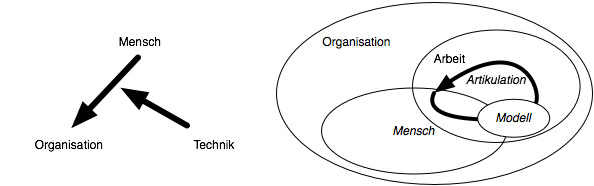
\includegraphics[width=15cm]{img/ExkursMOT/untersuchungsgegenstand.png}
	\caption{Untersuchungsgegenstände}
	\label{fig:img_untersuchungsgegenstand}
\end{figure}

In den folgenden Absätzen werden nun die einzelnen Untersuchungsgegenstände detailliert und in das „MOT“-System eingeordnet. Zusammenfassen kann gesagt werden, dass untersucht wird, welche Auswirkungen der Einsatz von Modellen für arbeitende Menschen bei der Artikulation ihrer individuellen Sicht auf ihre Arbeit hat und wie dieser 

\paragraph{Modell} % (fold)
\label{par:modell}

Modelle (also diagrammatische Repräsentationen) von Arbeit werden in dieser Arbeit eingesetzt, um Individuen (\emph{M}) ihre Arbeit (\emph{O}) -- also jene organisationalen Abläufe in die sie involviert sind, sowie deren Kontext -- abzubilden. Modelle sind hier also individuelle Instrumente, die verwendet werden, um organisationale Phänomene zu beschreiben. In diesem Zusammenhang ist zu untersuchen, welche Eigenschaft die Repräsentationsform der Modelle aufweisen muss, um die Repräsentierbarkeit beliebiger individueller Sichten in Modellen gewährleisten zu können. Dies entspricht im wesentlichen der Beziehung zwischen \emph{M} und \emph{O} in Abbildung \ref{fig:img_untersuchungsgegenstand}.
% paragraph modell (end)

\paragraph{Mensch} % (fold)
\label{par:mensch}

Der Mensch (\emph{M}) als Träger von Arbeit (d.h. als ausführende Instanz) und gleichzeitig als artikulierende (d.h. im Kontext dieser Arbeit: modellierende) Instanz steht im Zentrum der Betrachtungen dieser Arbeit. Untersucht werden muss, wie Menschen Modelle von Arbeit erstellen (können), wie sie diese interpretieren und welche Anforderungen sowohl aus organisationaler (\emph{O}) als auch aus technischer (\emph{T}) Sicht jeweils erfüllt sein müssen, um diese Abläufe zu unterstützen. Dies entspricht im wesentlichen dem Knoten \emph{M} in Abbildung \ref{fig:img_untersuchungsgegenstand}.

% paragraph mensch (end)

\paragraph{Artikulation} % (fold)
\label{par:artikulation}

Als Artikulation wird jener Vorgang bezeichnet, bei dem Menschen (\emph{M}) individuell oder kollektiv ihre Sichten auf ihre Arbeit (\emph{O}) reflektieren und ggf. anpassen bzw. abstimmen -- dieser Prozess ist gleichzeitig integraler Bestandteil von Arbeit selbst. Hier wird einerseits untersucht, wie dieser Artikulationsprozess durch den Einsatz von Modellen (diagrammatischen Repräsentationen) ermöglicht bzw. erleichtert wird und wie die Erstellung der Modelle technisch (T) unterstützt werden kann. Dies entspricht im wesentlichen der Beziehung zwischen \emph{T} und der Kante \emph{M-O} in Abbildung \ref{fig:img_untersuchungsgegenstand}. Zusätzlich ist zu untersuchen, wie sich die Arbeit (\emph{O}) aus Sicht der handelnden Menschen (\emph{M}) durch die Artikulation verändert hat.

% paragraph artikulation (end)
% chapter methodik (end)